\documentclass[1p]{elsarticle_modified}
%\bibliographystyle{elsarticle-num}

%\usepackage[colorlinks]{hyperref}
%\usepackage{abbrmath_seonhwa} %\Abb, \Ascr, \Acal ,\Abf, \Afrak
\usepackage{amsfonts}
\usepackage{amssymb}
\usepackage{amsmath}
\usepackage{amsthm}
\usepackage{scalefnt}
\usepackage{amsbsy}
\usepackage{kotex}
\usepackage{caption}
\usepackage{subfig}
\usepackage{color}
\usepackage{graphicx}
\usepackage{xcolor} %% white, black, red, green, blue, cyan, magenta, yellow
\usepackage{float}
\usepackage{setspace}
\usepackage{hyperref}

\usepackage{tikz}
\usetikzlibrary{arrows}

\usepackage{multirow}
\usepackage{array} % fixed length table
\usepackage{hhline}

%%%%%%%%%%%%%%%%%%%%%
\makeatletter
\renewcommand*\env@matrix[1][\arraystretch]{%
	\edef\arraystretch{#1}%
	\hskip -\arraycolsep
	\let\@ifnextchar\new@ifnextchar
	\array{*\c@MaxMatrixCols c}}
\makeatother %https://tex.stackexchange.com/questions/14071/how-can-i-increase-the-line-spacing-in-a-matrix
%%%%%%%%%%%%%%%

\usepackage[normalem]{ulem}

\newcommand{\msout}[1]{\ifmmode\text{\sout{\ensuremath{#1}}}\else\sout{#1}\fi}
%SOURCE: \msout is \stkout macro in https://tex.stackexchange.com/questions/20609/strikeout-in-math-mode

\newcommand{\cancel}[1]{
	\ifmmode
	{\color{red}\msout{#1}}
	\else
	{\color{red}\sout{#1}}
	\fi
}

\newcommand{\add}[1]{
	{\color{blue}\uwave{#1}}
}

\newcommand{\replace}[2]{
	\ifmmode
	{\color{red}\msout{#1}}{\color{blue}\uwave{#2}}
	\else
	{\color{red}\sout{#1}}{\color{blue}\uwave{#2}}
	\fi
}

\newcommand{\Sol}{\mathcal{S}} %segment
\newcommand{\D}{D} %diagram
\newcommand{\A}{\mathcal{A}} %arc


%%%%%%%%%%%%%%%%%%%%%%%%%%%%%5 test

\def\sl{\operatorname{\textup{SL}}(2,\Cbb)}
\def\psl{\operatorname{\textup{PSL}}(2,\Cbb)}
\def\quan{\mkern 1mu \triangleright \mkern 1mu}

\theoremstyle{definition}
\newtheorem{thm}{Theorem}[section]
\newtheorem{prop}[thm]{Proposition}
\newtheorem{lem}[thm]{Lemma}
\newtheorem{ques}[thm]{Question}
\newtheorem{cor}[thm]{Corollary}
\newtheorem{defn}[thm]{Definition}
\newtheorem{exam}[thm]{Example}
\newtheorem{rmk}[thm]{Remark}
\newtheorem{alg}[thm]{Algorithm}

\newcommand{\I}{\sqrt{-1}}
\begin{document}

%\begin{frontmatter}
%
%\title{Boundary parabolic representations of knots up to 8 crossings}
%
%%% Group authors per affiliation:
%\author{Yunhi Cho} 
%\address{Department of Mathematics, University of Seoul, Seoul, Korea}
%\ead{yhcho@uos.ac.kr}
%
%
%\author{Seonhwa Kim} %\fnref{s_kim}}
%\address{Center for Geometry and Physics, Institute for Basic Science, Pohang, 37673, Korea}
%\ead{ryeona17@ibs.re.kr}
%
%\author{Hyuk Kim}
%\address{Department of Mathematical Sciences, Seoul National University, Seoul 08826, Korea}
%\ead{hyukkim@snu.ac.kr}
%
%\author{Seokbeom Yoon}
%\address{Department of Mathematical Sciences, Seoul National University, Seoul, 08826,  Korea}
%\ead{sbyoon15@snu.ac.kr}
%
%\begin{abstract}
%We find all boundary parabolic representation of knots up to 8 crossings.
%
%\end{abstract}
%\begin{keyword}
%    \MSC[2010] 57M25 
%\end{keyword}
%
%\end{frontmatter}

%\linenumbers
%\tableofcontents
%
\newcommand\colored[1]{\textcolor{white}{\rule[-0.35ex]{0.8em}{1.4ex}}\kern-0.8em\color{red} #1}%
%\newcommand\colored[1]{\textcolor{white}{ #1}\kern-2.17ex	\textcolor{white}{ #1}\kern-1.81ex	\textcolor{white}{ #1}\kern-2.15ex\color{red}#1	}

{\Large $\underline{12n_{0512}~(K12n_{0512})}$}

\setlength{\tabcolsep}{10pt}
\renewcommand{\arraystretch}{1.6}
\vspace{1cm}\begin{tabular}{m{100pt}>{\centering\arraybackslash}m{274pt}}
\multirow{5}{120pt}{
	\centering
	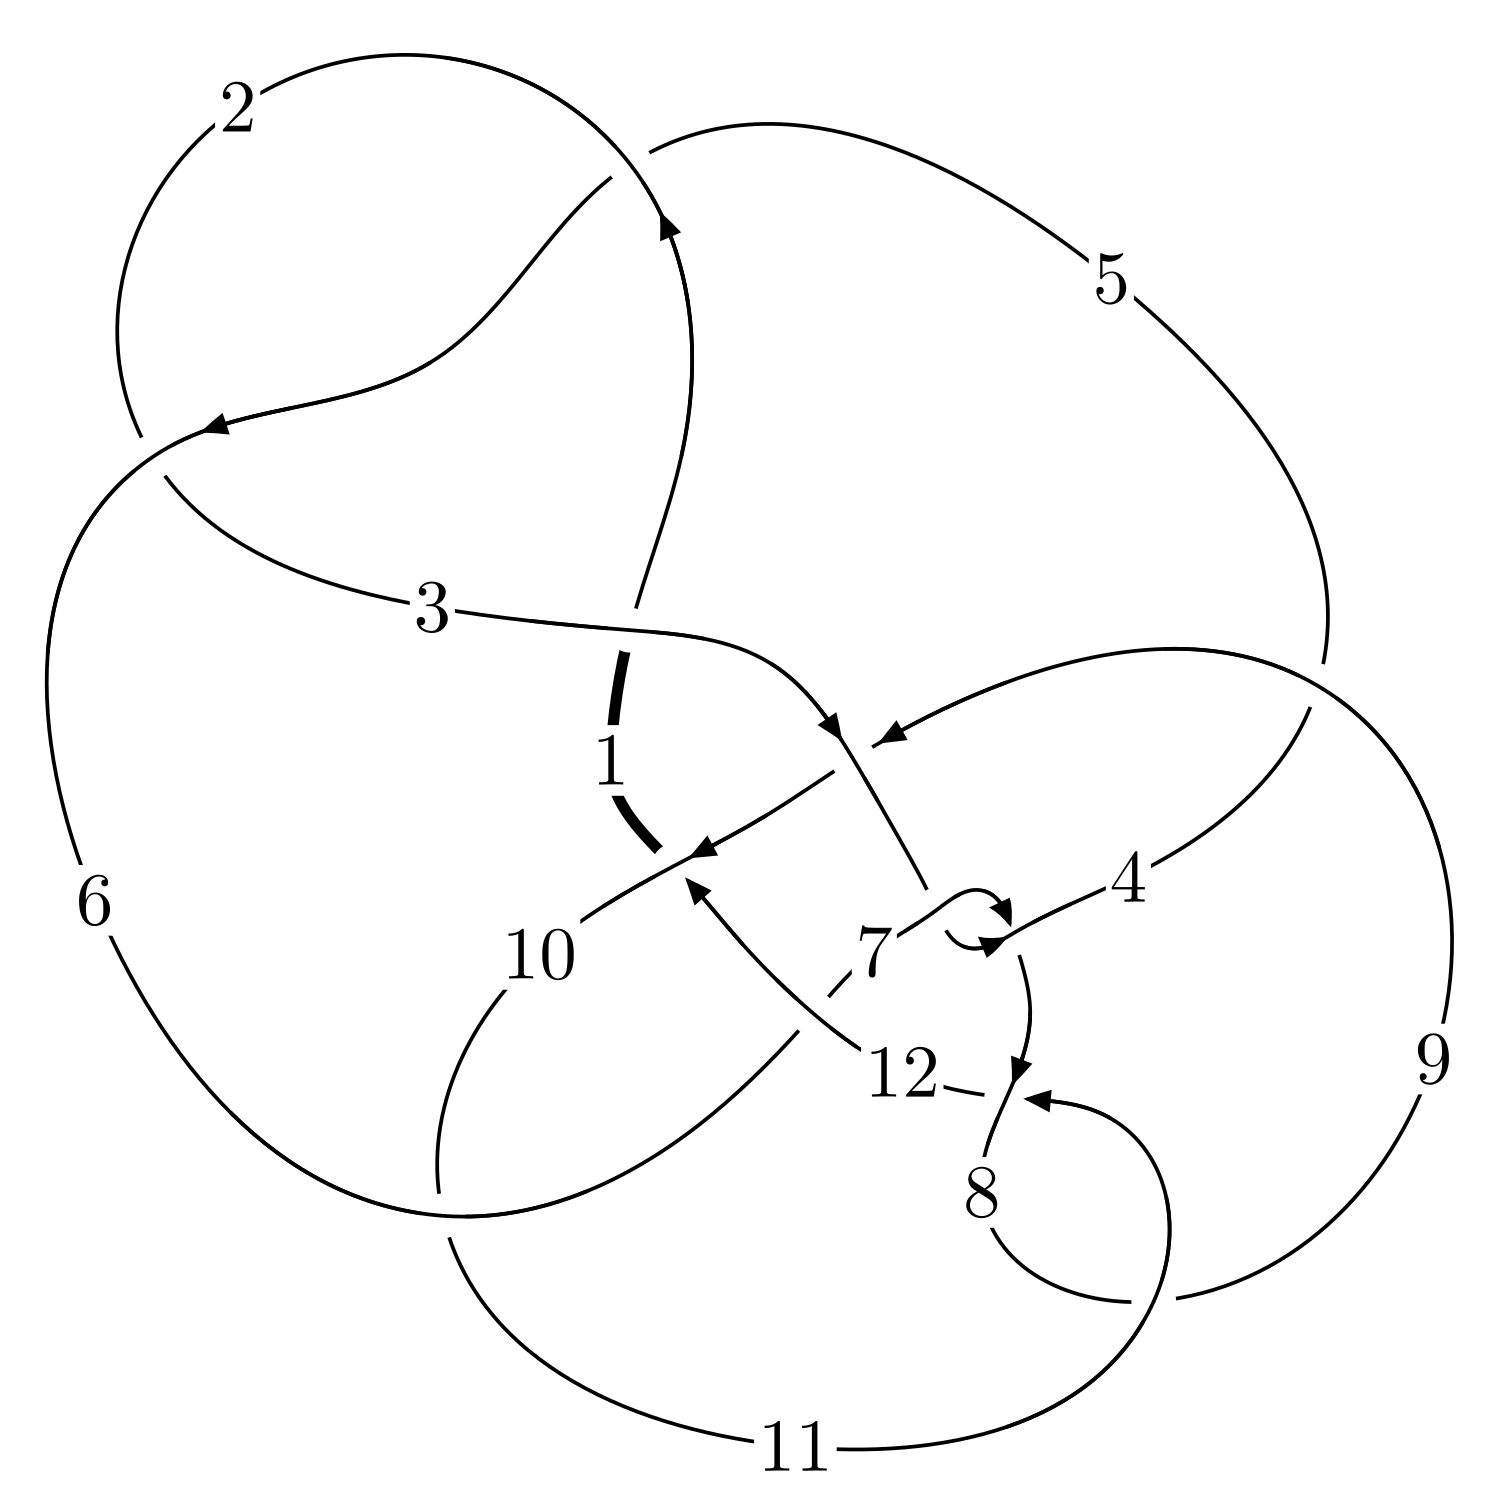
\includegraphics[width=112pt]{../../../GIT/diagram.site/Diagrams/png/2601_12n_0512.png}\\
\ \ \ A knot diagram\footnotemark}&
\allowdisplaybreaks
\textbf{Linearized knot diagam} \\
\cline{2-2}
 &
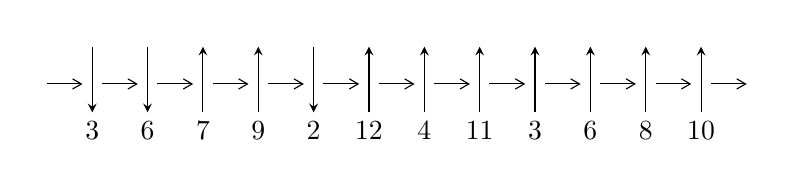
\begin{tikzpicture}[x=20pt, y=17pt]
	% nodes
	\node (C0) at (0, 0) {};
	\node (C1) at (1, 0) {};
	\node (C1U) at (1, +1) {};
	\node (C1D) at (1, -1) {3};

	\node (C2) at (2, 0) {};
	\node (C2U) at (2, +1) {};
	\node (C2D) at (2, -1) {6};

	\node (C3) at (3, 0) {};
	\node (C3U) at (3, +1) {};
	\node (C3D) at (3, -1) {7};

	\node (C4) at (4, 0) {};
	\node (C4U) at (4, +1) {};
	\node (C4D) at (4, -1) {9};

	\node (C5) at (5, 0) {};
	\node (C5U) at (5, +1) {};
	\node (C5D) at (5, -1) {2};

	\node (C6) at (6, 0) {};
	\node (C6U) at (6, +1) {};
	\node (C6D) at (6, -1) {12};

	\node (C7) at (7, 0) {};
	\node (C7U) at (7, +1) {};
	\node (C7D) at (7, -1) {4};

	\node (C8) at (8, 0) {};
	\node (C8U) at (8, +1) {};
	\node (C8D) at (8, -1) {11};

	\node (C9) at (9, 0) {};
	\node (C9U) at (9, +1) {};
	\node (C9D) at (9, -1) {3};

	\node (C10) at (10, 0) {};
	\node (C10U) at (10, +1) {};
	\node (C10D) at (10, -1) {6};

	\node (C11) at (11, 0) {};
	\node (C11U) at (11, +1) {};
	\node (C11D) at (11, -1) {8};

	\node (C12) at (12, 0) {};
	\node (C12U) at (12, +1) {};
	\node (C12D) at (12, -1) {10};
	\node (C13) at (13, 0) {};

	% arrows
	\draw[->,>={angle 60}]
	(C0) edge (C1) (C1) edge (C2) (C2) edge (C3) (C3) edge (C4) (C4) edge (C5) (C5) edge (C6) (C6) edge (C7) (C7) edge (C8) (C8) edge (C9) (C9) edge (C10) (C10) edge (C11) (C11) edge (C12) (C12) edge (C13) ;	\draw[->,>=stealth]
	(C1U) edge (C1D) (C2U) edge (C2D) (C3D) edge (C3U) (C4D) edge (C4U) (C5U) edge (C5D) (C6D) edge (C6U) (C7D) edge (C7U) (C8D) edge (C8U) (C9D) edge (C9U) (C10D) edge (C10U) (C11D) edge (C11U) (C12D) edge (C12U) ;
	\end{tikzpicture} \\
\hhline{~~} \\& 
\textbf{Solving Sequence} \\ \cline{2-2} 
 &
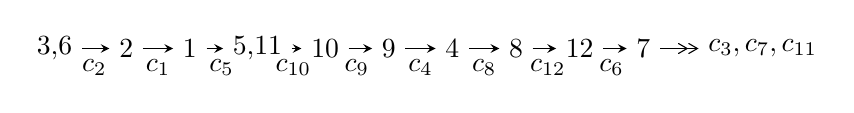
\begin{tikzpicture}[x=23pt, y=7pt]
	% node
	\node (A0) at (-1/8, 0) {3,6};
	\node (A1) at (1, 0) {2};
	\node (A2) at (2, 0) {1};
	\node (A3) at (49/16, 0) {5,11};
	\node (A4) at (33/8, 0) {10};
	\node (A5) at (41/8, 0) {9};
	\node (A6) at (49/8, 0) {4};
	\node (A7) at (57/8, 0) {8};
	\node (A8) at (65/8, 0) {12};
	\node (A9) at (73/8, 0) {7};
	\node (C1) at (1/2, -1) {$c_{2}$};
	\node (C2) at (3/2, -1) {$c_{1}$};
	\node (C3) at (5/2, -1) {$c_{5}$};
	\node (C4) at (29/8, -1) {$c_{10}$};
	\node (C5) at (37/8, -1) {$c_{9}$};
	\node (C6) at (45/8, -1) {$c_{4}$};
	\node (C7) at (53/8, -1) {$c_{8}$};
	\node (C8) at (61/8, -1) {$c_{12}$};
	\node (C9) at (69/8, -1) {$c_{6}$};
	\node (A10) at (11, 0) {$c_{3},c_{7},c_{11}$};

	% edge
	\draw[->,>=stealth]	
	(A0) edge (A1) (A1) edge (A2) (A2) edge (A3) (A3) edge (A4) (A4) edge (A5) (A5) edge (A6) (A6) edge (A7) (A7) edge (A8) (A8) edge (A9) ;
	\draw[->>,>={angle 60}]	
	(A9) edge (A10);
\end{tikzpicture} \\ 

\end{tabular} \\

\footnotetext{
The image of knot diagram is generated by the software ``\textbf{Draw programme}" developed by Andrew Bartholomew(\url{http://www.layer8.co.uk/maths/draw/index.htm\#Running-draw}), where we modified some parts for our purpose(\url{https://github.com/CATsTAILs/LinksPainter}).
}\phantom \\ \newline 
\centering \textbf{Ideals for irreducible components\footnotemark of $X_{\text{par}}$} 
 
\begin{align*}
I^u_{1}&=\langle 
-3.56209\times10^{137} u^{52}+2.13565\times10^{138} u^{51}+\cdots+5.27502\times10^{137} b-7.84392\times10^{138},\\
\phantom{I^u_{1}}&\phantom{= \langle  }-1.41680\times10^{139} u^{52}+8.65355\times10^{139} u^{51}+\cdots+5.27502\times10^{137} a-1.27431\times10^{140},\\
\phantom{I^u_{1}}&\phantom{= \langle  }u^{53}-6 u^{52}+\cdots+40 u+1\rangle \\
I^u_{2}&=\langle 
-457327227 u^{19}-610703148 u^{18}+\cdots+96358259 b+1111419337,\\
\phantom{I^u_{2}}&\phantom{= \langle  }2105382800 u^{19}+2179873747 u^{18}+\cdots+1252657367 a-8679007382,\;u^{20}+u^{19}+\cdots-3 u+1\rangle \\
\\
\end{align*}
\raggedright * 2 irreducible components of $\dim_{\mathbb{C}}=0$, with total 73 representations.\\
\footnotetext{All coefficients of polynomials are rational numbers. But the coefficients are sometimes approximated in decimal forms when there is not enough margin.}
\newpage
\renewcommand{\arraystretch}{1}
\centering \section*{I. $I^u_{1}= \langle -3.56\times10^{137} u^{52}+2.14\times10^{138} u^{51}+\cdots+5.28\times10^{137} b-7.84\times10^{138},\;-1.42\times10^{139} u^{52}+8.65\times10^{139} u^{51}+\cdots+5.28\times10^{137} a-1.27\times10^{140},\;u^{53}-6 u^{52}+\cdots+40 u+1 \rangle$}
\flushleft \textbf{(i) Arc colorings}\\
\begin{tabular}{m{7pt} m{180pt} m{7pt} m{180pt} }
\flushright $a_{3}=$&$\begin{pmatrix}1\\0\end{pmatrix}$ \\
\flushright $a_{6}=$&$\begin{pmatrix}0\\u\end{pmatrix}$ \\
\flushright $a_{2}=$&$\begin{pmatrix}1\\- u^2\end{pmatrix}$ \\
\flushright $a_{1}=$&$\begin{pmatrix}- u^2+1\\- u^2\end{pmatrix}$ \\
\flushright $a_{5}=$&$\begin{pmatrix}u\\- u^3+u\end{pmatrix}$ \\
\flushright $a_{11}=$&$\begin{pmatrix}26.8586 u^{52}-164.048 u^{51}+\cdots+7449.00 u+241.575\\0.675274 u^{52}-4.04861 u^{51}+\cdots+369.847 u+14.8699\end{pmatrix}$ \\
\flushright $a_{10}=$&$\begin{pmatrix}26.8586 u^{52}-164.048 u^{51}+\cdots+7449.00 u+241.575\\0.965646 u^{52}-5.81779 u^{51}+\cdots+458.826 u+17.7659\end{pmatrix}$ \\
\flushright $a_{9}=$&$\begin{pmatrix}25.8930 u^{52}-158.230 u^{51}+\cdots+6990.17 u+223.809\\0.965646 u^{52}-5.81779 u^{51}+\cdots+458.826 u+17.7659\end{pmatrix}$ \\
\flushright $a_{4}=$&$\begin{pmatrix}-18.4782 u^{52}+112.605 u^{51}+\cdots-6257.19 u-224.169\\1.57008 u^{52}-9.59238 u^{51}+\cdots+487.147 u+16.3474\end{pmatrix}$ \\
\flushright $a_{8}=$&$\begin{pmatrix}-2.77482 u^{52}+16.5932 u^{51}+\cdots-1230.46 u-34.8505\\-1.36325 u^{52}+8.33041 u^{51}+\cdots-410.734 u-14.9305\end{pmatrix}$ \\
\flushright $a_{12}=$&$\begin{pmatrix}21.3342 u^{52}-129.983 u^{51}+\cdots+6833.05 u+226.930\\3.27322 u^{52}-19.9309 u^{51}+\cdots+1054.12 u+37.4865\end{pmatrix}$ \\
\flushright $a_{7}=$&$\begin{pmatrix}19.9047 u^{52}-121.176 u^{51}+\cdots+6787.17 u+238.652\\-0.884196 u^{52}+5.40601 u^{51}+\cdots-268.684 u-8.40868\end{pmatrix}$\\&\end{tabular}
\flushleft \textbf{(ii) Obstruction class $= -1$}\\~\\
\flushleft \textbf{(iii) Cusp Shapes $= 40.2182 u^{52}-245.280 u^{51}+\cdots+12382.7 u+427.694$}\\~\\
\newpage\renewcommand{\arraystretch}{1}
\flushleft \textbf{(iv) u-Polynomials at the component}\newline \\
\begin{tabular}{m{50pt}|m{274pt}}
Crossings & \hspace{64pt}u-Polynomials at each crossing \\
\hline $$\begin{aligned}c_{1}\end{aligned}$$&$\begin{aligned}
&u^{53}+80 u^{52}+\cdots+238 u+1
\end{aligned}$\\
\hline $$\begin{aligned}c_{2},c_{5}\end{aligned}$$&$\begin{aligned}
&u^{53}+6 u^{52}+\cdots+40 u-1
\end{aligned}$\\
\hline $$\begin{aligned}c_{3},c_{7}\end{aligned}$$&$\begin{aligned}
&u^{53}-17 u^{51}+\cdots+63 u-11
\end{aligned}$\\
\hline $$\begin{aligned}c_{4}\end{aligned}$$&$\begin{aligned}
&u^{53}+u^{52}+\cdots-131614 u-3089431
\end{aligned}$\\
\hline $$\begin{aligned}c_{6}\end{aligned}$$&$\begin{aligned}
&u^{53}-2 u^{52}+\cdots-45 u-25
\end{aligned}$\\
\hline $$\begin{aligned}c_{8},c_{11}\end{aligned}$$&$\begin{aligned}
&u^{53}+7 u^{52}+\cdots-392 u-37
\end{aligned}$\\
\hline $$\begin{aligned}c_{9}\end{aligned}$$&$\begin{aligned}
&u^{53}-2 u^{52}+\cdots+34266 u-3617
\end{aligned}$\\
\hline $$\begin{aligned}c_{10}\end{aligned}$$&$\begin{aligned}
&u^{53}+7 u^{52}+\cdots+22602191 u-16425077
\end{aligned}$\\
\hline $$\begin{aligned}c_{12}\end{aligned}$$&$\begin{aligned}
&u^{53}+u^{52}+\cdots+528726 u-213397
\end{aligned}$\\
\hline
\end{tabular}\\~\\
\newpage\renewcommand{\arraystretch}{1}
\flushleft \textbf{(v) Riley Polynomials at the component}\newline \\
\begin{tabular}{m{50pt}|m{274pt}}
Crossings & \hspace{64pt}Riley Polynomials at each crossing \\
\hline $$\begin{aligned}c_{1}\end{aligned}$$&$\begin{aligned}
&y^{53}-212 y^{52}+\cdots+14210 y-1
\end{aligned}$\\
\hline $$\begin{aligned}c_{2},c_{5}\end{aligned}$$&$\begin{aligned}
&y^{53}-80 y^{52}+\cdots+238 y-1
\end{aligned}$\\
\hline $$\begin{aligned}c_{3},c_{7}\end{aligned}$$&$\begin{aligned}
&y^{53}-34 y^{52}+\cdots+3309 y-121
\end{aligned}$\\
\hline $$\begin{aligned}c_{4}\end{aligned}$$&$\begin{aligned}
&y^{53}+55 y^{52}+\cdots-87460058633830 y-9544583903761
\end{aligned}$\\
\hline $$\begin{aligned}c_{6}\end{aligned}$$&$\begin{aligned}
&y^{53}+8 y^{52}+\cdots-16775 y-625
\end{aligned}$\\
\hline $$\begin{aligned}c_{8},c_{11}\end{aligned}$$&$\begin{aligned}
&y^{53}+41 y^{52}+\cdots+12250 y-1369
\end{aligned}$\\
\hline $$\begin{aligned}c_{9}\end{aligned}$$&$\begin{aligned}
&y^{53}+102 y^{52}+\cdots+1220203166 y-13082689
\end{aligned}$\\
\hline $$\begin{aligned}c_{10}\end{aligned}$$&$\begin{aligned}
&y^{53}+71 y^{52}+\cdots-2845499866554563 y-269783154455929
\end{aligned}$\\
\hline $$\begin{aligned}c_{12}\end{aligned}$$&$\begin{aligned}
&y^{53}+93 y^{52}+\cdots-373137198832 y-45538279609
\end{aligned}$\\
\hline
\end{tabular}\\~\\
\newpage\flushleft \textbf{(vi) Complex Volumes and Cusp Shapes}
$$\begin{array}{c|c|c}  
\text{Solutions to }I^u_{1}& \I (\text{vol} + \sqrt{-1}CS) & \text{Cusp shape}\\
 \hline 
\begin{aligned}
u &= -0.651411 + 0.752062 I \\
a &= -1.134320 + 0.061409 I \\
b &= -0.511145 - 0.535779 I\end{aligned}
 & -3.88667 - 1.27131 I & \phantom{-0.000000 } 0 \\ \hline\begin{aligned}
u &= -0.651411 - 0.752062 I \\
a &= -1.134320 - 0.061409 I \\
b &= -0.511145 + 0.535779 I\end{aligned}
 & -3.88667 + 1.27131 I & \phantom{-0.000000 } 0 \\ \hline\begin{aligned}
u &= \phantom{-}0.992728 + 0.033495 I \\
a &= \phantom{-}1.012130 - 0.339700 I \\
b &= -1.193880 - 0.568300 I\end{aligned}
 & \phantom{-}0.238785 - 0.926241 I & \phantom{-0.000000 } 0 \\ \hline\begin{aligned}
u &= \phantom{-}0.992728 - 0.033495 I \\
a &= \phantom{-}1.012130 + 0.339700 I \\
b &= -1.193880 + 0.568300 I\end{aligned}
 & \phantom{-}0.238785 + 0.926241 I & \phantom{-0.000000 } 0 \\ \hline\begin{aligned}
u &= \phantom{-}1.010360 + 0.207032 I \\
a &= -0.585032 - 0.713094 I \\
b &= -0.373601 - 0.012887 I\end{aligned}
 & -3.66107 - 0.98999 I & \phantom{-0.000000 } 0 \\ \hline\begin{aligned}
u &= \phantom{-}1.010360 - 0.207032 I \\
a &= -0.585032 + 0.713094 I \\
b &= -0.373601 + 0.012887 I\end{aligned}
 & -3.66107 + 0.98999 I & \phantom{-0.000000 } 0 \\ \hline\begin{aligned}
u &= -0.834510 + 0.668017 I \\
a &= -0.037971 + 0.804259 I \\
b &= -0.811369 + 0.481691 I\end{aligned}
 & \phantom{-}1.21719 + 5.26322 I & \phantom{-0.000000 } 0 \\ \hline\begin{aligned}
u &= -0.834510 - 0.668017 I \\
a &= -0.037971 - 0.804259 I \\
b &= -0.811369 - 0.481691 I\end{aligned}
 & \phantom{-}1.21719 - 5.26322 I & \phantom{-0.000000 } 0 \\ \hline\begin{aligned}
u &= \phantom{-}0.827402 + 0.388907 I \\
a &= \phantom{-}0.140688 - 0.616647 I \\
b &= -0.620881 - 0.428477 I\end{aligned}
 & -1.43824 - 1.25865 I & \phantom{-0.000000 } 0 \\ \hline\begin{aligned}
u &= \phantom{-}0.827402 - 0.388907 I \\
a &= \phantom{-}0.140688 + 0.616647 I \\
b &= -0.620881 + 0.428477 I\end{aligned}
 & -1.43824 + 1.25865 I & \phantom{-0.000000 } 0\\
 \hline 
 \end{array}$$\newpage$$\begin{array}{c|c|c}  
\text{Solutions to }I^u_{1}& \I (\text{vol} + \sqrt{-1}CS) & \text{Cusp shape}\\
 \hline 
\begin{aligned}
u &= -0.581625 + 0.702705 I \\
a &= \phantom{-}0.846217 - 0.114913 I \\
b &= \phantom{-}0.347803 + 0.705862 I\end{aligned}
 & \phantom{-}2.02336 - 0.17363 I & \phantom{-0.000000 } 0 \\ \hline\begin{aligned}
u &= -0.581625 - 0.702705 I \\
a &= \phantom{-}0.846217 + 0.114913 I \\
b &= \phantom{-}0.347803 - 0.705862 I\end{aligned}
 & \phantom{-}2.02336 + 0.17363 I & \phantom{-0.000000 } 0 \\ \hline\begin{aligned}
u &= -0.604136 + 0.653648 I \\
a &= \phantom{-}0.15330 - 2.45151 I \\
b &= \phantom{-}2.94062 - 1.54125 I\end{aligned}
 & -1.09785 - 5.39717 I & \phantom{-0.000000 } 0 \\ \hline\begin{aligned}
u &= -0.604136 - 0.653648 I \\
a &= \phantom{-}0.15330 + 2.45151 I \\
b &= \phantom{-}2.94062 + 1.54125 I\end{aligned}
 & -1.09785 + 5.39717 I & \phantom{-0.000000 } 0 \\ \hline\begin{aligned}
u &= -0.234994 + 0.792616 I \\
a &= -0.68335 + 1.25161 I \\
b &= -0.967724 + 0.802230 I\end{aligned}
 & \phantom{-}0.64524 - 2.29715 I & \phantom{-0.000000 } 0 \\ \hline\begin{aligned}
u &= -0.234994 - 0.792616 I \\
a &= -0.68335 - 1.25161 I \\
b &= -0.967724 - 0.802230 I\end{aligned}
 & \phantom{-}0.64524 + 2.29715 I & \phantom{-0.000000 } 0 \\ \hline\begin{aligned}
u &= \phantom{-}1.011050 + 0.728145 I \\
a &= -0.863583 - 0.230870 I \\
b &= -0.209639 + 0.531099 I\end{aligned}
 & -2.58796 + 4.29315 I & \phantom{-0.000000 } 0 \\ \hline\begin{aligned}
u &= \phantom{-}1.011050 - 0.728145 I \\
a &= -0.863583 + 0.230870 I \\
b &= -0.209639 - 0.531099 I\end{aligned}
 & -2.58796 - 4.29315 I & \phantom{-0.000000 } 0 \\ \hline\begin{aligned}
u &= -0.722480 + 0.177433 I \\
a &= -1.08346 + 1.04580 I \\
b &= -0.530116 - 0.093427 I\end{aligned}
 & -4.43015 - 2.75918 I & \phantom{-0.000000 -}0. + 6.84222 I \\ \hline\begin{aligned}
u &= -0.722480 - 0.177433 I \\
a &= -1.08346 - 1.04580 I \\
b &= -0.530116 + 0.093427 I\end{aligned}
 & -4.43015 + 2.75918 I & \phantom{-0.000000 } 0. - 6.84222 I\\
 \hline 
 \end{array}$$\newpage$$\begin{array}{c|c|c}  
\text{Solutions to }I^u_{1}& \I (\text{vol} + \sqrt{-1}CS) & \text{Cusp shape}\\
 \hline 
\begin{aligned}
u &= -0.656788 + 0.104423 I \\
a &= \phantom{-}1.139030 - 0.753059 I \\
b &= -1.035190 + 0.001812 I\end{aligned}
 & \phantom{-}1.75452 + 1.11434 I & \phantom{-}6.66980 - 0.91738 I \\ \hline\begin{aligned}
u &= -0.656788 - 0.104423 I \\
a &= \phantom{-}1.139030 + 0.753059 I \\
b &= -1.035190 - 0.001812 I\end{aligned}
 & \phantom{-}1.75452 - 1.11434 I & \phantom{-}6.66980 + 0.91738 I \\ \hline\begin{aligned}
u &= \phantom{-}1.19055 + 0.88568 I \\
a &= \phantom{-}1.03039 + 1.18794 I \\
b &= \phantom{-}3.01001 - 2.00642 I\end{aligned}
 & -5.54516 - 2.28770 I & \phantom{-0.000000 } 0 \\ \hline\begin{aligned}
u &= \phantom{-}1.19055 - 0.88568 I \\
a &= \phantom{-}1.03039 - 1.18794 I \\
b &= \phantom{-}3.01001 + 2.00642 I\end{aligned}
 & -5.54516 + 2.28770 I & \phantom{-0.000000 } 0 \\ \hline\begin{aligned}
u &= -1.25052 + 0.95834 I \\
a &= \phantom{-}0.765795 - 0.742774 I \\
b &= \phantom{-}1.93360 + 1.56424 I\end{aligned}
 & -2.29349 + 8.62681 I & \phantom{-0.000000 } 0 \\ \hline\begin{aligned}
u &= -1.25052 - 0.95834 I \\
a &= \phantom{-}0.765795 + 0.742774 I \\
b &= \phantom{-}1.93360 - 1.56424 I\end{aligned}
 & -2.29349 - 8.62681 I & \phantom{-0.000000 } 0 \\ \hline\begin{aligned}
u &= \phantom{-}0.015951 + 0.307510 I \\
a &= -3.13764 - 2.41335 I \\
b &= -1.067820 - 0.221770 I\end{aligned}
 & -2.76658 - 2.41535 I & \phantom{-}4.47087 + 1.33196 I \\ \hline\begin{aligned}
u &= \phantom{-}0.015951 - 0.307510 I \\
a &= -3.13764 + 2.41335 I \\
b &= -1.067820 + 0.221770 I\end{aligned}
 & -2.76658 + 2.41535 I & \phantom{-}4.47087 - 1.33196 I \\ \hline\begin{aligned}
u &= \phantom{-}1.73290 + 0.22179 I \\
a &= -0.166376 + 0.891503 I \\
b &= \phantom{-}1.53471 - 0.39631 I\end{aligned}
 & -13.03680 + 0.42178 I & \phantom{-0.000000 } 0 \\ \hline\begin{aligned}
u &= \phantom{-}1.73290 - 0.22179 I \\
a &= -0.166376 - 0.891503 I \\
b &= \phantom{-}1.53471 + 0.39631 I\end{aligned}
 & -13.03680 - 0.42178 I & \phantom{-0.000000 } 0\\
 \hline 
 \end{array}$$\newpage$$\begin{array}{c|c|c}  
\text{Solutions to }I^u_{1}& \I (\text{vol} + \sqrt{-1}CS) & \text{Cusp shape}\\
 \hline 
\begin{aligned}
u &= -0.222604\phantom{ +0.000000I} \\
a &= \phantom{-}2.63595\phantom{ +0.000000I} \\
b &= \phantom{-}0.204967\phantom{ +0.000000I}\end{aligned}
 & \phantom{-}0.751427\phantom{ +0.000000I} & \phantom{-}13.9310\phantom{ +0.000000I} \\ \hline\begin{aligned}
u &= \phantom{-}1.79232 + 0.08357 I \\
a &= -0.253542 + 0.882171 I \\
b &= \phantom{-}0.692163 - 0.475817 I\end{aligned}
 & -8.36557 - 7.93433 I & \phantom{-0.000000 } 0 \\ \hline\begin{aligned}
u &= \phantom{-}1.79232 - 0.08357 I \\
a &= -0.253542 - 0.882171 I \\
b &= \phantom{-}0.692163 + 0.475817 I\end{aligned}
 & -8.36557 + 7.93433 I & \phantom{-0.000000 } 0 \\ \hline\begin{aligned}
u &= -1.81353 + 0.16616 I \\
a &= -0.207496 - 0.844861 I \\
b &= \phantom{-}1.317620 + 0.423194 I\end{aligned}
 & -13.8162 + 3.3112 I & \phantom{-0.000000 } 0 \\ \hline\begin{aligned}
u &= -1.81353 - 0.16616 I \\
a &= -0.207496 + 0.844861 I \\
b &= \phantom{-}1.317620 - 0.423194 I\end{aligned}
 & -13.8162 - 3.3112 I & \phantom{-0.000000 } 0 \\ \hline\begin{aligned}
u &= \phantom{-}1.82641 + 0.02277 I \\
a &= -0.408438 - 0.956178 I \\
b &= \phantom{-}0.835144 + 1.106430 I\end{aligned}
 & -7.20845 - 1.41990 I & \phantom{-0.000000 } 0 \\ \hline\begin{aligned}
u &= \phantom{-}1.82641 - 0.02277 I \\
a &= -0.408438 + 0.956178 I \\
b &= \phantom{-}0.835144 - 1.106430 I\end{aligned}
 & -7.20845 + 1.41990 I & \phantom{-0.000000 } 0 \\ \hline\begin{aligned}
u &= -1.83249 + 0.05934 I \\
a &= -0.289698 - 0.861622 I \\
b &= \phantom{-}0.850502 + 0.649158 I\end{aligned}
 & -11.49160 + 3.02837 I & \phantom{-0.000000 } 0 \\ \hline\begin{aligned}
u &= -1.83249 - 0.05934 I \\
a &= -0.289698 + 0.861622 I \\
b &= \phantom{-}0.850502 - 0.649158 I\end{aligned}
 & -11.49160 - 3.02837 I & \phantom{-0.000000 } 0 \\ \hline\begin{aligned}
u &= -0.0831788 + 0.0833293 I \\
a &= \phantom{-}9.86402 - 1.69209 I \\
b &= -1.031690 + 0.055942 I\end{aligned}
 & \phantom{-}0.30393 - 7.10088 I & \phantom{-}6.36388 + 5.33035 I\\
 \hline 
 \end{array}$$\newpage$$\begin{array}{c|c|c}  
\text{Solutions to }I^u_{1}& \I (\text{vol} + \sqrt{-1}CS) & \text{Cusp shape}\\
 \hline 
\begin{aligned}
u &= -0.0831788 - 0.0833293 I \\
a &= \phantom{-}9.86402 + 1.69209 I \\
b &= -1.031690 - 0.055942 I\end{aligned}
 & \phantom{-}0.30393 + 7.10088 I & \phantom{-}6.36388 - 5.33035 I \\ \hline\begin{aligned}
u &= -0.0934579 + 0.0087537 I \\
a &= -4.09016 + 5.62846 I \\
b &= \phantom{-}1.230780 + 0.270711 I\end{aligned}
 & \phantom{-}3.45336 - 0.72834 I & \phantom{-}4.97850 + 9.73372 I \\ \hline\begin{aligned}
u &= -0.0934579 - 0.0087537 I \\
a &= -4.09016 - 5.62846 I \\
b &= \phantom{-}1.230780 - 0.270711 I\end{aligned}
 & \phantom{-}3.45336 + 0.72834 I & \phantom{-}4.97850 - 9.73372 I \\ \hline\begin{aligned}
u &= \phantom{-}1.92828 + 0.39816 I \\
a &= -0.073932 + 0.751779 I \\
b &= \phantom{-}1.55124 - 0.77066 I\end{aligned}
 & -12.70340 - 4.46357 I & \phantom{-0.000000 } 0 \\ \hline\begin{aligned}
u &= \phantom{-}1.92828 - 0.39816 I \\
a &= -0.073932 - 0.751779 I \\
b &= \phantom{-}1.55124 + 0.77066 I\end{aligned}
 & -12.70340 + 4.46357 I & \phantom{-0.000000 } 0 \\ \hline\begin{aligned}
u &= \phantom{-}1.95974 + 0.27409 I \\
a &= \phantom{-}0.495203 - 1.120220 I \\
b &= -2.64977 + 1.35321 I\end{aligned}
 & -13.4569 - 14.5302 I & \phantom{-0.000000 } 0 \\ \hline\begin{aligned}
u &= \phantom{-}1.95974 - 0.27409 I \\
a &= \phantom{-}0.495203 + 1.120220 I \\
b &= -2.64977 - 1.35321 I\end{aligned}
 & -13.4569 + 14.5302 I & \phantom{-0.000000 } 0 \\ \hline\begin{aligned}
u &= -1.96062 + 0.27144 I \\
a &= \phantom{-}0.606172 + 1.255340 I \\
b &= -3.13934 - 1.65634 I\end{aligned}
 & -16.6143 + 7.9534 I & \phantom{-0.000000 } 0 \\ \hline\begin{aligned}
u &= -1.96062 - 0.27144 I \\
a &= \phantom{-}0.606172 - 1.255340 I \\
b &= -3.13934 + 1.65634 I\end{aligned}
 & -16.6143 - 7.9534 I & \phantom{-0.000000 } 0 \\ \hline\begin{aligned}
u &= -1.99808 + 0.23948 I \\
a &= -0.171286 - 0.721049 I \\
b &= \phantom{-}1.35791 + 0.78829 I\end{aligned}
 & -13.38850 + 1.15104 I & \phantom{-0.000000 } 0\\
 \hline 
 \end{array}$$\newpage$$\begin{array}{c|c|c}  
\text{Solutions to }I^u_{1}& \I (\text{vol} + \sqrt{-1}CS) & \text{Cusp shape}\\
 \hline 
\begin{aligned}
u &= -1.99808 - 0.23948 I \\
a &= -0.171286 + 0.721049 I \\
b &= \phantom{-}1.35791 - 0.78829 I\end{aligned}
 & -13.38850 - 1.15104 I & \phantom{-0.000000 } 0 \\ \hline\begin{aligned}
u &= \phantom{-}2.14143 + 0.40086 I \\
a &= \phantom{-}1.31536 - 2.28235 I \\
b &= -8.56241 + 4.52922 I\end{aligned}
 & -9.57518 - 1.18543 I & \phantom{-0.000000 } 0 \\ \hline\begin{aligned}
u &= \phantom{-}2.14143 - 0.40086 I \\
a &= \phantom{-}1.31536 + 2.28235 I \\
b &= -8.56241 - 4.52922 I\end{aligned}
 & -9.57518 + 1.18543 I & \phantom{-0.000000 } 0\\
 \hline 
 \end{array}$$\newpage\newpage\renewcommand{\arraystretch}{1}
\centering \section*{II. $I^u_{2}= \langle -4.57\times10^{8} u^{19}-6.11\times10^{8} u^{18}+\cdots+9.64\times10^{7} b+1.11\times10^{9},\;2.11\times10^{9} u^{19}+2.18\times10^{9} u^{18}+\cdots+1.25\times10^{9} a-8.68\times10^{9},\;u^{20}+u^{19}+\cdots-3 u+1 \rangle$}
\flushleft \textbf{(i) Arc colorings}\\
\begin{tabular}{m{7pt} m{180pt} m{7pt} m{180pt} }
\flushright $a_{3}=$&$\begin{pmatrix}1\\0\end{pmatrix}$ \\
\flushright $a_{6}=$&$\begin{pmatrix}0\\u\end{pmatrix}$ \\
\flushright $a_{2}=$&$\begin{pmatrix}1\\- u^2\end{pmatrix}$ \\
\flushright $a_{1}=$&$\begin{pmatrix}- u^2+1\\- u^2\end{pmatrix}$ \\
\flushright $a_{5}=$&$\begin{pmatrix}u\\- u^3+u\end{pmatrix}$ \\
\flushright $a_{11}=$&$\begin{pmatrix}-1.68073 u^{19}-1.74020 u^{18}+\cdots+1.22079 u+6.92848\\4.74611 u^{19}+6.33784 u^{18}+\cdots+4.25754 u-11.5342\end{pmatrix}$ \\
\flushright $a_{10}=$&$\begin{pmatrix}-1.68073 u^{19}-1.74020 u^{18}+\cdots+1.22079 u+6.92848\\4.92880 u^{19}+6.87890 u^{18}+\cdots+5.75988 u-11.4748\end{pmatrix}$ \\
\flushright $a_{9}=$&$\begin{pmatrix}-6.60953 u^{19}-8.61910 u^{18}+\cdots-4.53908 u+18.4033\\4.92880 u^{19}+6.87890 u^{18}+\cdots+5.75988 u-11.4748\end{pmatrix}$ \\
\flushright $a_{4}=$&$\begin{pmatrix}17.7080 u^{19}+25.0549 u^{18}+\cdots+26.1497 u-42.8331\\-5.23321 u^{19}-7.65134 u^{18}+\cdots-8.10067 u+11.1686\end{pmatrix}$ \\
\flushright $a_{8}=$&$\begin{pmatrix}2.92468 u^{19}+5.21610 u^{18}+\cdots+12.4614 u-3.29960\\3.04593 u^{19}+4.28134 u^{18}+\cdots+2.39110 u-8.17378\end{pmatrix}$ \\
\flushright $a_{12}=$&$\begin{pmatrix}9.53421 u^{19}+13.8352 u^{18}+\cdots+17.0004 u-19.7029\\2.01703 u^{19}+2.81058 u^{18}+\cdots+0.239552 u-5.24907\end{pmatrix}$ \\
\flushright $a_{7}=$&$\begin{pmatrix}18.3525 u^{19}+26.1833 u^{18}+\cdots+30.0756 u-42.2405\\-2.82962 u^{19}-4.30100 u^{18}+\cdots-5.11549 u+5.70458\end{pmatrix}$\\&\end{tabular}
\flushleft \textbf{(ii) Obstruction class $= 1$}\\~\\
\flushleft \textbf{(iii) Cusp Shapes $= -\frac{16130734190}{1252657367} u^{19}-\frac{21563499972}{1252657367} u^{18}+\cdots-\frac{38299165429}{1252657367} u+\frac{44038168311}{1252657367}$}\\~\\
\newpage\renewcommand{\arraystretch}{1}
\flushleft \textbf{(iv) u-Polynomials at the component}\newline \\
\begin{tabular}{m{50pt}|m{274pt}}
Crossings & \hspace{64pt}u-Polynomials at each crossing \\
\hline $$\begin{aligned}c_{1}\end{aligned}$$&$\begin{aligned}
&u^{20}-23 u^{19}+\cdots-21 u+1
\end{aligned}$\\
\hline $$\begin{aligned}c_{2}\end{aligned}$$&$\begin{aligned}
&u^{20}+u^{19}+\cdots-3 u+1
\end{aligned}$\\
\hline $$\begin{aligned}c_{3}\end{aligned}$$&$\begin{aligned}
&u^{20}-3 u^{19}+\cdots-2 u+1
\end{aligned}$\\
\hline $$\begin{aligned}c_{4}\end{aligned}$$&$\begin{aligned}
&u^{20}+6 u^{18}+\cdots+9 u+1
\end{aligned}$\\
\hline $$\begin{aligned}c_{5}\end{aligned}$$&$\begin{aligned}
&u^{20}- u^{19}+\cdots+3 u+1
\end{aligned}$\\
\hline $$\begin{aligned}c_{6}\end{aligned}$$&$\begin{aligned}
&u^{20}- u^{19}+\cdots-4 u+1
\end{aligned}$\\
\hline $$\begin{aligned}c_{7}\end{aligned}$$&$\begin{aligned}
&u^{20}+3 u^{19}+\cdots+2 u+1
\end{aligned}$\\
\hline $$\begin{aligned}c_{8}\end{aligned}$$&$\begin{aligned}
&u^{20}+6 u^{19}+\cdots+45 u+7
\end{aligned}$\\
\hline $$\begin{aligned}c_{9}\end{aligned}$$&$\begin{aligned}
&u^{20}- u^{19}+\cdots- u+1
\end{aligned}$\\
\hline $$\begin{aligned}c_{10}\end{aligned}$$&$\begin{aligned}
&u^{20}+4 u^{19}+\cdots+4 u+1
\end{aligned}$\\
\hline $$\begin{aligned}c_{11}\end{aligned}$$&$\begin{aligned}
&u^{20}-6 u^{19}+\cdots-45 u+7
\end{aligned}$\\
\hline $$\begin{aligned}c_{12}\end{aligned}$$&$\begin{aligned}
&u^{20}+9 u^{18}+\cdots+u+1
\end{aligned}$\\
\hline
\end{tabular}\\~\\
\newpage\renewcommand{\arraystretch}{1}
\flushleft \textbf{(v) Riley Polynomials at the component}\newline \\
\begin{tabular}{m{50pt}|m{274pt}}
Crossings & \hspace{64pt}Riley Polynomials at each crossing \\
\hline $$\begin{aligned}c_{1}\end{aligned}$$&$\begin{aligned}
&y^{20}-51 y^{19}+\cdots-41 y+1
\end{aligned}$\\
\hline $$\begin{aligned}c_{2},c_{5}\end{aligned}$$&$\begin{aligned}
&y^{20}-23 y^{19}+\cdots-21 y+1
\end{aligned}$\\
\hline $$\begin{aligned}c_{3},c_{7}\end{aligned}$$&$\begin{aligned}
&y^{20}-17 y^{19}+\cdots-16 y+1
\end{aligned}$\\
\hline $$\begin{aligned}c_{4}\end{aligned}$$&$\begin{aligned}
&y^{20}+12 y^{19}+\cdots-61 y+1
\end{aligned}$\\
\hline $$\begin{aligned}c_{6}\end{aligned}$$&$\begin{aligned}
&y^{20}+y^{19}+\cdots-16 y+1
\end{aligned}$\\
\hline $$\begin{aligned}c_{8},c_{11}\end{aligned}$$&$\begin{aligned}
&y^{20}+14 y^{19}+\cdots+215 y+49
\end{aligned}$\\
\hline $$\begin{aligned}c_{9}\end{aligned}$$&$\begin{aligned}
&y^{20}+23 y^{19}+\cdots-5 y+1
\end{aligned}$\\
\hline $$\begin{aligned}c_{10}\end{aligned}$$&$\begin{aligned}
&y^{20}+20 y^{19}+\cdots-4 y+1
\end{aligned}$\\
\hline $$\begin{aligned}c_{12}\end{aligned}$$&$\begin{aligned}
&y^{20}+18 y^{19}+\cdots-7 y+1
\end{aligned}$\\
\hline
\end{tabular}\\~\\
\newpage\flushleft \textbf{(vi) Complex Volumes and Cusp Shapes}
$$\begin{array}{c|c|c}  
\text{Solutions to }I^u_{2}& \I (\text{vol} + \sqrt{-1}CS) & \text{Cusp shape}\\
 \hline 
\begin{aligned}
u &= -0.953168 + 0.477953 I \\
a &= \phantom{-}0.027910 - 0.764739 I \\
b &= \phantom{-}1.43070 + 0.64601 I\end{aligned}
 & -0.15553 + 8.95849 I & \phantom{-}6.05677 - 7.79186 I \\ \hline\begin{aligned}
u &= -0.953168 - 0.477953 I \\
a &= \phantom{-}0.027910 + 0.764739 I \\
b &= \phantom{-}1.43070 - 0.64601 I\end{aligned}
 & -0.15553 - 8.95849 I & \phantom{-}6.05677 + 7.79186 I \\ \hline\begin{aligned}
u &= \phantom{-}1.076970 + 0.113176 I \\
a &= \phantom{-}0.644492 - 0.140096 I \\
b &= -1.051310 - 0.246752 I\end{aligned}
 & -0.753541 - 0.108333 I & \phantom{-}1.89880 - 1.85099 I \\ \hline\begin{aligned}
u &= \phantom{-}1.076970 - 0.113176 I \\
a &= \phantom{-}0.644492 + 0.140096 I \\
b &= -1.051310 + 0.246752 I\end{aligned}
 & -0.753541 + 0.108333 I & \phantom{-}1.89880 + 1.85099 I \\ \hline\begin{aligned}
u &= -0.880029 + 0.788989 I \\
a &= -0.483386 + 0.858602 I \\
b &= -1.96510 + 0.09601 I\end{aligned}
 & \phantom{-}0.01293 - 4.36454 I & \phantom{-}5.65242 + 3.34145 I \\ \hline\begin{aligned}
u &= -0.880029 - 0.788989 I \\
a &= -0.483386 - 0.858602 I \\
b &= -1.96510 - 0.09601 I\end{aligned}
 & \phantom{-}0.01293 + 4.36454 I & \phantom{-}5.65242 - 3.34145 I \\ \hline\begin{aligned}
u &= \phantom{-}0.573843 + 0.568398 I \\
a &= -1.211620 - 0.162641 I \\
b &= -0.560549 + 0.039344 I\end{aligned}
 & -3.66684 + 1.94633 I & \phantom{-}5.45415 - 4.37772 I \\ \hline\begin{aligned}
u &= \phantom{-}0.573843 - 0.568398 I \\
a &= -1.211620 + 0.162641 I \\
b &= -0.560549 - 0.039344 I\end{aligned}
 & -3.66684 - 1.94633 I & \phantom{-}5.45415 + 4.37772 I \\ \hline\begin{aligned}
u &= \phantom{-}0.735779 + 0.317158 I \\
a &= -0.35138 + 1.55614 I \\
b &= \phantom{-}1.399420 - 0.144993 I\end{aligned}
 & -3.47476 - 3.31570 I & \phantom{-}0.67932 + 5.99198 I \\ \hline\begin{aligned}
u &= \phantom{-}0.735779 - 0.317158 I \\
a &= -0.35138 - 1.55614 I \\
b &= \phantom{-}1.399420 + 0.144993 I\end{aligned}
 & -3.47476 + 3.31570 I & \phantom{-}0.67932 - 5.99198 I\\
 \hline 
 \end{array}$$\newpage$$\begin{array}{c|c|c}  
\text{Solutions to }I^u_{2}& \I (\text{vol} + \sqrt{-1}CS) & \text{Cusp shape}\\
 \hline 
\begin{aligned}
u &= -1.165200 + 0.433501 I \\
a &= \phantom{-}0.353048 + 0.390155 I \\
b &= -1.45248 + 0.46098 I\end{aligned}
 & \phantom{-}1.34131 + 3.38449 I & \phantom{-}4.71773 - 3.89524 I \\ \hline\begin{aligned}
u &= -1.165200 - 0.433501 I \\
a &= \phantom{-}0.353048 - 0.390155 I \\
b &= -1.45248 - 0.46098 I\end{aligned}
 & \phantom{-}1.34131 - 3.38449 I & \phantom{-}4.71773 + 3.89524 I \\ \hline\begin{aligned}
u &= -0.466533 + 0.291062 I \\
a &= \phantom{-}0.540211 - 0.115052 I \\
b &= \phantom{-}0.937438 + 0.236499 I\end{aligned}
 & \phantom{-}3.58769 - 0.13487 I & \phantom{-}11.02112 - 2.80092 I \\ \hline\begin{aligned}
u &= -0.466533 - 0.291062 I \\
a &= \phantom{-}0.540211 + 0.115052 I \\
b &= \phantom{-}0.937438 - 0.236499 I\end{aligned}
 & \phantom{-}3.58769 + 0.13487 I & \phantom{-}11.02112 + 2.80092 I \\ \hline\begin{aligned}
u &= \phantom{-}0.418981 + 0.040038 I \\
a &= \phantom{-}2.42239 - 0.52074 I \\
b &= -0.469495 + 1.066240 I\end{aligned}
 & -1.05506 + 2.08410 I & \phantom{-}2.22198 - 2.68803 I \\ \hline\begin{aligned}
u &= \phantom{-}0.418981 - 0.040038 I \\
a &= \phantom{-}2.42239 + 0.52074 I \\
b &= -0.469495 - 1.066240 I\end{aligned}
 & -1.05506 - 2.08410 I & \phantom{-}2.22198 + 2.68803 I \\ \hline\begin{aligned}
u &= -1.88694 + 0.23384 I \\
a &= -0.168220 - 0.691711 I \\
b &= \phantom{-}1.315960 + 0.356311 I\end{aligned}
 & -12.85410 + 2.44827 I & \phantom{-}4.74569 - 1.68433 I \\ \hline\begin{aligned}
u &= -1.88694 - 0.23384 I \\
a &= -0.168220 + 0.691711 I \\
b &= \phantom{-}1.315960 - 0.356311 I\end{aligned}
 & -12.85410 - 2.44827 I & \phantom{-}4.74569 + 1.68433 I \\ \hline\begin{aligned}
u &= \phantom{-}2.04630 + 0.30975 I \\
a &= -0.77344 + 1.85675 I \\
b &= \phantom{-}4.91542 - 3.72104 I\end{aligned}
 & -9.30106 - 1.00549 I & \phantom{-}8.05201 - 4.41716 I \\ \hline\begin{aligned}
u &= \phantom{-}2.04630 - 0.30975 I \\
a &= -0.77344 - 1.85675 I \\
b &= \phantom{-}4.91542 + 3.72104 I\end{aligned}
 & -9.30106 + 1.00549 I & \phantom{-}8.05201 + 4.41716 I\\
 \hline 
 \end{array}$$\newpage
\newpage\renewcommand{\arraystretch}{1}
\centering \section*{ III. u-Polynomials}
\begin{tabular}{m{50pt}|m{274pt}}
Crossings & \hspace{64pt}u-Polynomials at each crossing \\
\hline $$\begin{aligned}c_{1}\end{aligned}$$&$\begin{aligned}
&(u^{20}-23 u^{19}+\cdots-21 u+1)(u^{53}+80 u^{52}+\cdots+238 u+1)
\end{aligned}$\\
\hline $$\begin{aligned}c_{2}\end{aligned}$$&$\begin{aligned}
&(u^{20}+u^{19}+\cdots-3 u+1)(u^{53}+6 u^{52}+\cdots+40 u-1)
\end{aligned}$\\
\hline $$\begin{aligned}c_{3}\end{aligned}$$&$\begin{aligned}
&(u^{20}-3 u^{19}+\cdots-2 u+1)(u^{53}-17 u^{51}+\cdots+63 u-11)
\end{aligned}$\\
\hline $$\begin{aligned}c_{4}\end{aligned}$$&$\begin{aligned}
&(u^{20}+6 u^{18}+\cdots+9 u+1)(u^{53}+u^{52}+\cdots-131614 u-3089431)
\end{aligned}$\\
\hline $$\begin{aligned}c_{5}\end{aligned}$$&$\begin{aligned}
&(u^{20}- u^{19}+\cdots+3 u+1)(u^{53}+6 u^{52}+\cdots+40 u-1)
\end{aligned}$\\
\hline $$\begin{aligned}c_{6}\end{aligned}$$&$\begin{aligned}
&(u^{20}- u^{19}+\cdots-4 u+1)(u^{53}-2 u^{52}+\cdots-45 u-25)
\end{aligned}$\\
\hline $$\begin{aligned}c_{7}\end{aligned}$$&$\begin{aligned}
&(u^{20}+3 u^{19}+\cdots+2 u+1)(u^{53}-17 u^{51}+\cdots+63 u-11)
\end{aligned}$\\
\hline $$\begin{aligned}c_{8}\end{aligned}$$&$\begin{aligned}
&(u^{20}+6 u^{19}+\cdots+45 u+7)(u^{53}+7 u^{52}+\cdots-392 u-37)
\end{aligned}$\\
\hline $$\begin{aligned}c_{9}\end{aligned}$$&$\begin{aligned}
&(u^{20}- u^{19}+\cdots- u+1)(u^{53}-2 u^{52}+\cdots+34266 u-3617)
\end{aligned}$\\
\hline $$\begin{aligned}c_{10}\end{aligned}$$&$\begin{aligned}
&(u^{20}+4 u^{19}+\cdots+4 u+1)\\
&\cdot(u^{53}+7 u^{52}+\cdots+22602191 u-16425077)
\end{aligned}$\\
\hline $$\begin{aligned}c_{11}\end{aligned}$$&$\begin{aligned}
&(u^{20}-6 u^{19}+\cdots-45 u+7)(u^{53}+7 u^{52}+\cdots-392 u-37)
\end{aligned}$\\
\hline $$\begin{aligned}c_{12}\end{aligned}$$&$\begin{aligned}
&(u^{20}+9 u^{18}+\cdots+u+1)(u^{53}+u^{52}+\cdots+528726 u-213397)
\end{aligned}$\\
\hline
\end{tabular}\newpage\renewcommand{\arraystretch}{1}
\centering \section*{ IV. Riley Polynomials}
\begin{tabular}{m{50pt}|m{274pt}}
Crossings & \hspace{64pt}Riley Polynomials at each crossing \\
\hline $$\begin{aligned}c_{1}\end{aligned}$$&$\begin{aligned}
&(y^{20}-51 y^{19}+\cdots-41 y+1)(y^{53}-212 y^{52}+\cdots+14210 y-1)
\end{aligned}$\\
\hline $$\begin{aligned}c_{2},c_{5}\end{aligned}$$&$\begin{aligned}
&(y^{20}-23 y^{19}+\cdots-21 y+1)(y^{53}-80 y^{52}+\cdots+238 y-1)
\end{aligned}$\\
\hline $$\begin{aligned}c_{3},c_{7}\end{aligned}$$&$\begin{aligned}
&(y^{20}-17 y^{19}+\cdots-16 y+1)(y^{53}-34 y^{52}+\cdots+3309 y-121)
\end{aligned}$\\
\hline $$\begin{aligned}c_{4}\end{aligned}$$&$\begin{aligned}
&(y^{20}+12 y^{19}+\cdots-61 y+1)\\
&\cdot(y^{53}+55 y^{52}+\cdots-87460058633830 y-9544583903761)
\end{aligned}$\\
\hline $$\begin{aligned}c_{6}\end{aligned}$$&$\begin{aligned}
&(y^{20}+y^{19}+\cdots-16 y+1)(y^{53}+8 y^{52}+\cdots-16775 y-625)
\end{aligned}$\\
\hline $$\begin{aligned}c_{8},c_{11}\end{aligned}$$&$\begin{aligned}
&(y^{20}+14 y^{19}+\cdots+215 y+49)(y^{53}+41 y^{52}+\cdots+12250 y-1369)
\end{aligned}$\\
\hline $$\begin{aligned}c_{9}\end{aligned}$$&$\begin{aligned}
&(y^{20}+23 y^{19}+\cdots-5 y+1)\\
&\cdot(y^{53}+102 y^{52}+\cdots+1220203166 y-13082689)
\end{aligned}$\\
\hline $$\begin{aligned}c_{10}\end{aligned}$$&$\begin{aligned}
&(y^{20}+20 y^{19}+\cdots-4 y+1)\\
&\cdot(y^{53}+71 y^{52}+\cdots-2845499866554563 y-269783154455929)
\end{aligned}$\\
\hline $$\begin{aligned}c_{12}\end{aligned}$$&$\begin{aligned}
&(y^{20}+18 y^{19}+\cdots-7 y+1)\\
&\cdot(y^{53}+93 y^{52}+\cdots-373137198832 y-45538279609)
\end{aligned}$\\
\hline
\end{tabular}
\vskip 2pc
\end{document}